\section{Transposition}

It is simple to visualize the effect of transposing a matrix; it would be a rotation about the main diagonal. The resulting image will be rotated $90^\circ$. Taking the transpose again would give the original image orientation following the properties of transposed matrices:

    \[
    A=(A^T)^T
    \]

The effect can be seen in Figure~\ref{fig:tr}:

    \begin{figure}[h!]
        \centering
            \begin{subfigure}{0.3\textwidth}
                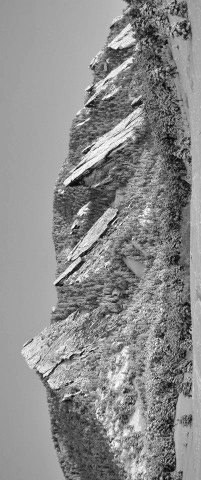
\includegraphics[scale=0.5]{./img/transpose1.png}
                \caption{Image 1 Transposed}
            \end{subfigure}
            \begin{subfigure}{0.3\textwidth}
                
\includegraphics[scale=0.5]{./img/transpose2.png}
                \caption{Image 2 Transposed}
            \end{subfigure}
        \caption{An example of a transposed image}
        \label{fig:tr}
    \end{figure}
